\documentclass[12pt]{article}
\usepackage[utf8]{inputenc}
\usepackage[spanish]{babel}
\usepackage{amsmath}
\usepackage{amsthm}
\usepackage{hyperref}
\usepackage{graphicx}
\usepackage{color}
\usepackage{float}
\usepackage{multicol}
\usepackage{enumerate}
\usepackage{anyfontsize}
\usepackage{anysize}
\usepackage{courier}
\usepackage{listingsutf8}
\usepackage{listings}
\usepackage{xcolor}
\usepackage{textcomp}
\usepackage{color}
\definecolor{deepblue}{rgb}{0,0,0.5}
\definecolor{brown}{rgb}{0.59, 0.29, 0.0}
\definecolor{OliveGreen}{rgb}{0,0.25,0}
% \usepackage{minted}

\DeclareCaptionFont{white}{\color{white}}
\DeclareCaptionFormat{listing}{\colorbox{gray}{\parbox{0.98\textwidth}{#1#2#3}}}
\captionsetup[lstlisting]{format=listing,labelfont=white,textfont=white}
\renewcommand{\lstlistingname}{Código}


\definecolor{Code}{rgb}{0,0,0}
\definecolor{Keywords}{rgb}{255,0,0}
\definecolor{Strings}{rgb}{255,0,255}
\definecolor{Comments}{rgb}{0,0,255}
\definecolor{Numbers}{rgb}{255,128,0}

\makeatletter

\newif\iffirstchar\firstchartrue
\newif\ifstartedbyadigit
\newif\ifprecededbyequalsign

\newcommand\processletter
{%
  \ifnum\lst@mode=\lst@Pmode%
    \iffirstchar%
        \global\startedbyadigitfalse%
      \fi
      \global\firstcharfalse%
    \fi
}

\newcommand\processdigit
{%
  \ifnum\lst@mode=\lst@Pmode%
      \iffirstchar%
        \global\startedbyadigittrue%
      \fi
      \global\firstcharfalse%
  \fi
}

\lst@AddToHook{OutputOther}%
{%
  \lst@IfLastOtherOneOf{=}
    {\global\precededbyequalsigntrue}
    {}%
}

\lst@AddToHook{Output}%
{%
  \ifprecededbyequalsign%
      \ifstartedbyadigit%
        \def\lst@thestyle{\color{orange}}%
      \fi
    \fi
  \global\firstchartrue%
  \global\startedbyadigitfalse%
  \global\precededbyequalsignfalse%
}

\lstset{ 
language=Python,                % choose the language of the code
basicstyle=\footnotesize\ttfamily,       % the size of the fonts that are used for the code
numbers=left,                   % where to put the line-numbers
numberstyle=\scriptsize,      % the size of the fonts that are used for the line-numbers
stepnumber=1,                   % the step between two line-numbers. If it is 1 each line will be numbered
numbersep=5pt,                  % how far the line-numbers are from the code
backgroundcolor=\color{white},  % choose the background color. You must add \usepackage{color}
showspaces=false,               % show spaces adding particular underscores
showstringspaces=false,         % underline spaces within strings
showtabs=false,                 % show tabs within strings adding particular underscores
frame=single,   		% adds a frame around the code
tabsize=2,  		% sets default tabsize to 2 spaces
captionpos=t,   		% sets the caption-position to bottom
breaklines=true,    	% sets automatic line breaking
breakatwhitespace=false,    % sets if automatic breaks should only happen at whitespace
escapeinside={\#},  % if you want to add a comment within your code
stringstyle =\color{OliveGreen},
%otherkeywords={{as}},             % Add keywords here
keywordstyle = \color{blue},
commentstyle = \color{black},
identifierstyle = \color{black},
literate=%
         {á}{{\'a}}1
         {é}{{\'e}}1
         {í}{{\'i}}1
         {ó}{{\'o}}1
         {ú}{{\'u}}1
%
%keywordstyle=\ttb\color{deepblue}
%fancyvrb = true,
}

\lstdefinestyle{FormattedNumber}{%
    literate={0}{{\textcolor{red}{0}}}{1}%
             {1}{{\textcolor{red}{1}}}{1}%
             {2}{{\textcolor{red}{2}}}{1}%
             {3}{{\textcolor{red}{3}}}{1}%
             {4}{{\textcolor{red}{4}}}{1}%
             {5}{{\textcolor{red}{5}}}{1}%
             {6}{{\textcolor{red}{6}}}{1}%
             {7}{{\textcolor{red}{7}}}{1}%
             {8}{{\textcolor{red}{8}}}{1}%
             {9}{{\textcolor{red}{9}}}{1}%
             {.0}{{\textcolor{red}{.0}}}{2}% Following is to ensure that only periods
             {.1}{{\textcolor{red}{.1}}}{2}% followed by a digit are changed.
             {.2}{{\textcolor{red}{.2}}}{2}%
             {.3}{{\textcolor{red}{.3}}}{2}%
             {.4}{{\textcolor{red}{.4}}}{2}%
             {.5}{{\textcolor{red}{.5}}}{2}%
             {.6}{{\textcolor{red}{.6}}}{2}%
             {.7}{{\textcolor{red}{.7}}}{2}%
             {.8}{{\textcolor{red}{.8}}}{2}%
             {.9}{{\textcolor{red}{.9}}}{2}%
             {\ }{{ }}{1}% handle the space
         ,%
          %mathescape=true
          escapeinside={__}
          }



\setlength{\parskip}{1em}
\spanishdecimal{.}
\renewcommand{\baselinestretch}{1.5}
\marginsize{1.5cm}{1.5cm}{1cm}{2cm}
\author{M. en C. Gustavo Contreras Mayén. \texttt{curso.fisica.comp@gmail.com}\\
M. en C. Abraham Lima Buendía. \texttt{abraham3081@ciencias.unam.mx}}
\title{Curso de Física Computacional}
\date{ }
\begin{document}
%\renewcommand\theenumii{\arabic{theenumii.enumii}}
\renewcommand\labelenumii{\theenumi.{\arabic{enumii}}}
\maketitle
\fontsize{14}{14}\selectfont
\section*{Ejercicio: Efecto de la resistencia del aire}
La bicicleta es una forma muy eficiente de transporte, este es un hecho bien conocido por cualquier persona que se sube en una. Nuestro objetivo en este ejercicio es comprender los factores que determinan la velocidad máxima de una bicicleta y estimar la velocidad de un caso real.
\par
Comenzaremos haciendo caso omiso de la fricción; tendremos que añadirlo al final, por supuesto, pero debemos primero entender cómo lidiar con el caso más simple y sin fricción.
\par
La ecuación de movimiento corresponde a la segunda ley de Newton, que escribimos de la forma
\begin{equation}
\dfrac{dv}{dt} = \dfrac{F}{m}
\label{EqNewton2}
\end{equation}
donde $v$ es la velocidad, $m$ es la masa de la combinación de la bicicleta-conductor, $t$ es el tiempo, y $F$ es la fuerza en la bicicleta que viene del esfuerzo del conductor (en este caso vamos a suponer que la bicicleta se mueve sobre un terreno plano)
\par
Tratar correctamente a $F$ se complica por la mecánica de la bicicleta, ya que la fuerza ejercida por el ciclista se transmite a las ruedas por medio del plato, engranajes, cadena, etc. Esto hace que sea muy difícil derivar una expresión exacta para $F$.
\par
Sin embargo, hay otra manera de abordar este problema que evita la necesidad de conocer la fuerza. Este enfoque alternativo implica la formulación del problema en términos de la potencia generada por el ciclista.
\par
Estudios fisiológicos de ciclistas de carreras han demostrado que estos atletas son capaces de producir una potencia de salida de aproximadamente 400 watts durante largos períodos de tiempo ($\sim 1$ h)
\par
Usando las ideas de trabajo-energía podemos reescribir (\ref{EqNewton2}) como
\begin{equation}\label{EqPotencia}
\dfrac{dE}{dt} = P
\end{equation}
donde $E$ es la energía total, $P$ es la potencia de salida del ciclista. Para un trayecto plano la energía es totalmente cinética, es decir, $E = \frac{1}{2} m v^{2}$, y $\frac{dE}{dt} = mv (\frac{dv}{dt})$, usando esto en (\ref{EqPotencia}), resulta
\begin{equation}\label{EqPotenciavel}
\dfrac{dv}{dt} = \dfrac{P}{mv}
\end{equation}
Si $P$ es una constante, la ecuación (\ref{EqPotenciavel}), se puede resolver de manera analítica, rearreglando términos:
\begin{equation}\label{EqIntegral}
\int_{v_{0}}^{v} v' dv' = \int_{0}^{t} \dfrac{P}{m} dt'
\end{equation}
donde $v_{0}$ es la velocidad de la bicicleta en $t=0$. Integrando ambos lados de la ecuación y resolviendo para $v$, tenemos
\begin{equation}\label{Eqvres}
v = \sqrt{v_{0}^{2} + 2 P \dfrac{t}{m}}
\end{equation}
Si bien esta es la solución correcta de la ecuación de movimiento (\ref{EqPotenciavel}), nuestro trabajo no concluye aquí, ya que predice que la velocidad se incrementará sin límite para tiempos muy largos.
\par
Vamos a corregir este resultado, cuando se generaliza el modelo se debe de incluir el efecto de la resistencia del aire. El nuevo término que vamos a añadir a la ecuación de movimiento nos obliga a desarrollar una solución numérica, así que con eso en mente se considera un tratamiento numérico de (\ref{EqPotenciavel})
\par
Comenzamos con la forma de diferencias finitas para la derivada de la velocidad
\begin{equation}\label{Eqderivada}
\dfrac{dv}{dt} \simeq \dfrac{v_{i+1}-v_{i}}{\Delta t}
\end{equation}
donde asumimos que $\Delta t$ es paso discreto pequeño, y $v_{i}$ es la velocidad al tiempo $t_{i} \equiv i \Delta t$, por lo que de la ecuación (\ref{EqPotenciavel})
\begin{equation}\label{Eqveli+1}
v_{i+1} = v_{i} + \dfrac{P}{m v_{i}} \Delta t
\end{equation}
Dada la velocidad en un tiempo $i$ (es decir, $v_{i}$), podemos usar (\ref{Eqveli+1}) para calcular un valor \textit{aproximado} de la velocidad en el siguiente paso $v_{i+1}$.
\par
Si conocemos la velocidad inicial $v_{0}$, podemos obtener $v_{1}$, $v_{2}$, y así sucesivamente.
Considera el siguiente código inicial
\begin{lstlisting}[basicstyle=\linespread{1.2}\ttfamily\small, columns=fullflexible,escapeinside=||]
import matplotlib.pyplot as plt
from math import sqrt

t = []
v = []

dt = 1

potencia = 400
masa = 70
tmax = 200
nmax = tmax/dt

t.append(0)
v.append(4)

for i in range(int(tmax/dt)):
    ti = t[i-1] + dt
    vi = sqrt(v[i]**2 + (2 * potencia * dt)/masa)
    
    
    t.append(ti)
    v.append(vi)

plt.plot(v, "r-")
plt.xlabel("tiempo [s]")
plt.ylabel("velocidad m/s")
plt.show()
\end{lstlisting}
Resultado de la velocidad sin fricción
\begin{figure}[H]
	\centering
	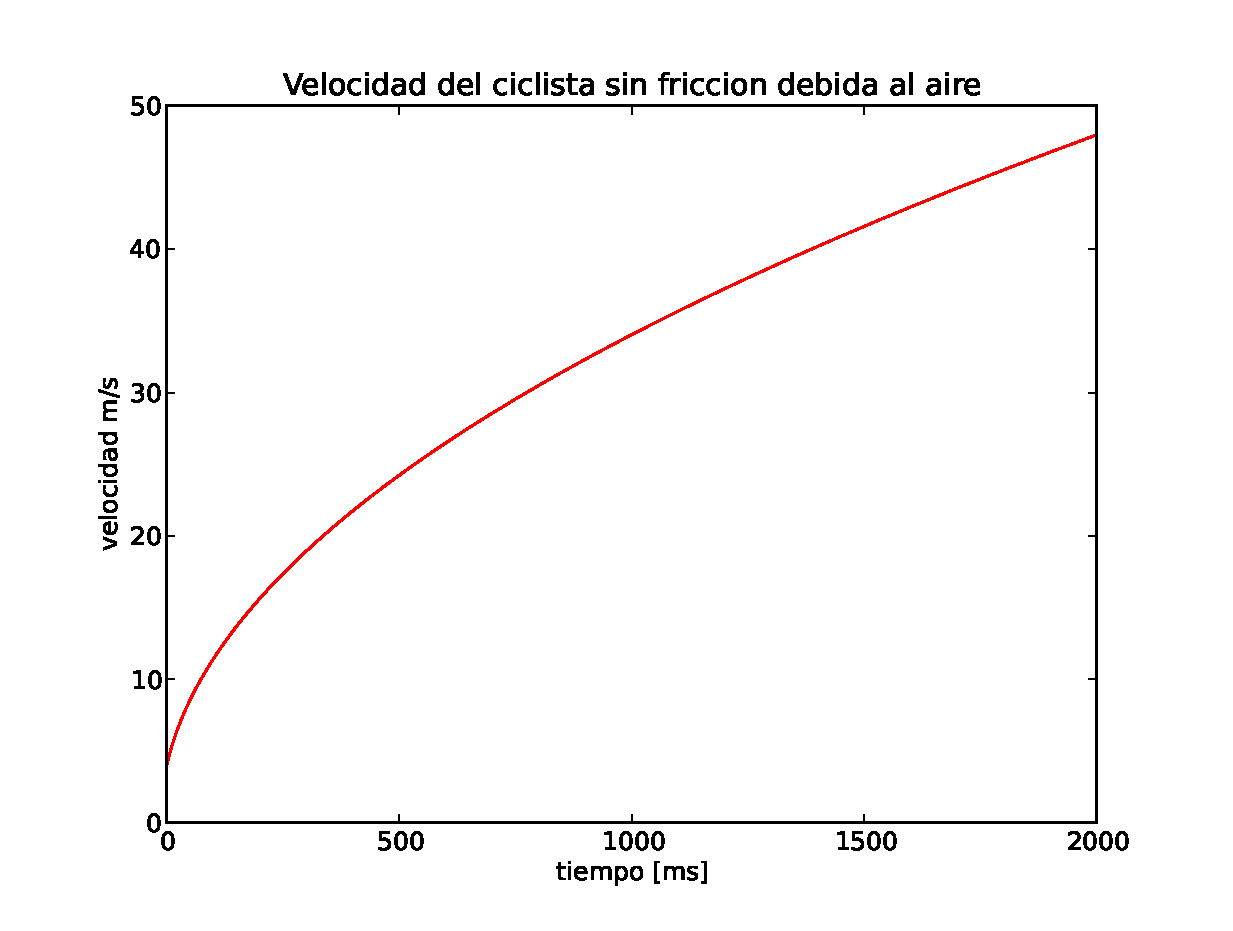
\includegraphics[scale=0.5]{EjerBicicleta01.eps}
\end{figure}

\section*{Considerando la fricción del aire}
La fuerza debida a la fricción puede aproximarse de manera inicial como
\begin{equation}\label{EqFfriccion}
F_{a} \simeq - B_{1} v - B_{2} v^{2}
\end{equation}
Para velocidades muy bajas, el primer término es el que domina, y el coeficiente $B_{1}$ se puede calcular para objetos con formas sencillas.
\par
Para una velocidad razonable $v^{2}$ el término domina sobre los demás, pero $B_{2}$ no puede calcularse exactamente en objetos sencillos como una pelota de beisbol, menos para una bicicleta.
\par
Podemos aproximar el valor de $B_{2}$ como sigue:
\par
Si un objeto se mueve a través de la atmósfera, debe empujar fuera del camino el aire delante de él. La masa de aire movido en el tiempo $dt$ es $m_{aire} \sim \rho A \: v \: dt$, donde $\rho$ es la densidad del aire y $A$ el área frontal del objeto. Este aire tiene una velocidad de orden $v$, y por lo tanto, su energía cinética es $E_{aire} \sim m_{aire} \: v^{2} /2$
\par
Este es también el trabajo realizado por la fuerza de arrastre (la fuerza sobre el objeto debido a la resistencia del aire) en el tiempo $dt$, por lo $F_{a} \: dt = E_{aire}$. Poniendo todo esto junto nos encontramos
\[ F_{a} \simeq - C \: \rho \: A \: v^{2} \]
Incluyendo este término en la expresión para la velocidad
\begin{equation}\label{Eqvelifriccion}
v_{i+1} = v_{i} + \dfrac{P}{m \: v_{i}} \Delta \: t - \dfrac{C \: \rho \: A \: v_{i}^{2}}{m} \: \Delta \: t
\end{equation}
Ahora te toca implementar el código, considerando $C = 0.5$ y $A=0.33$
\par
Comparando velocidades
\begin{figure}[H]
	\centering
	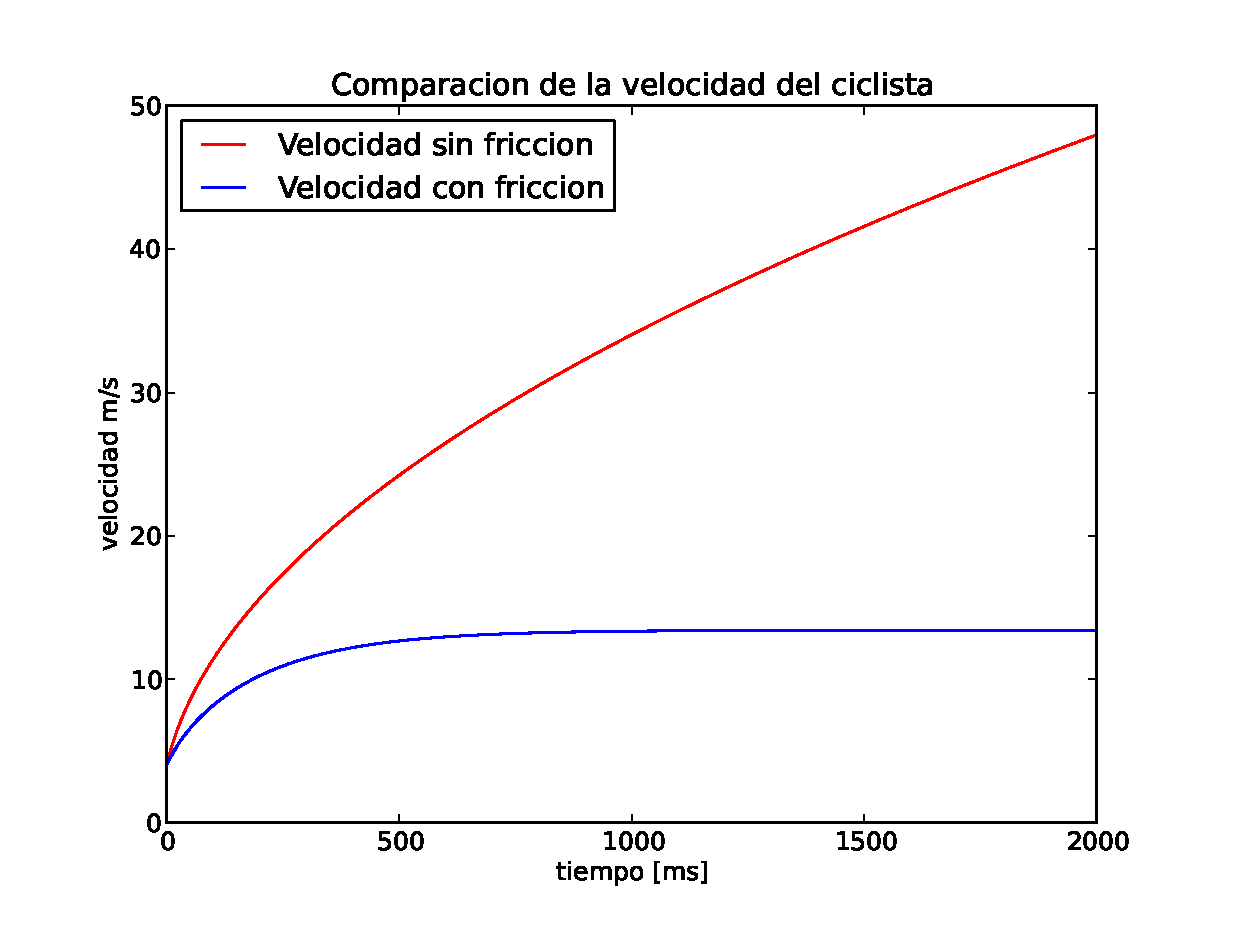
\includegraphics[scale=0.5]{EjerBicicleta02.eps}
\end{figure}
El resultado que tenemos a partir de nuestra solución numérica, es más congruente con la física. Nota que a pesar de tener un algoritmo que resuelve una ecuación de movimiento, nuestrto trabajo no termina con proporcionar una respuesta con el código, sino que revisemos la consistencia de la solución con la física que ya manejamos.
\end{document}